\chapter{Theoretical Aspects}
\label{chap:theoretical}

\myLettrine{S}{olar} power plants include multiple stages of converting the energy captured into varying voltage ranges and forms, either \gls{dc} or \gls{ac}, depending on the application that is used.
In general, these systems are integrated into the electrical grid infrastructure or used as power generators in the context of battery recharging or standalone operation in medium-sized industrial applications where the reliability on the traditional power infrastructures is rather poor. \cite{al2022photovoltaic}
\gls{pv} cells act as a \gls{dc} power source, but by themselves are insufficient for most practical applications, as they have to be connected in what is commonly known as solar panels, thus having different characteristics based on how these cells have been linked.
This usually leads to issues where the working characteristics of these panels have to be identified and mathematically modelled for efficient power conversion. \cite{al2022photovoltaic}
Additionally, the power output provided by these cells are affected by a multitude of external and internal factors, including, but not limited to:

\begin{itemize}
    \item Weather conditions, like rain, temperature and cloud coverage;
    \item Geographical positioning, as it reflects the maximum power available through solar irradiance;
    \item Cell degradation through aging of the internal p-n junction, thermal expansion and contraction, damaged induced by the elements (hailstone, winds carrying sand).
\end{itemize}

Thus, the power converted by these panels can vary drastically, and this variance in the input voltage provided by this source has to be accounted for when powering any load connected to the system.
A rough schematic of such system is included in \figref{fig:pvsystem}:

\begin{figure}[!ht]
    \begin{center}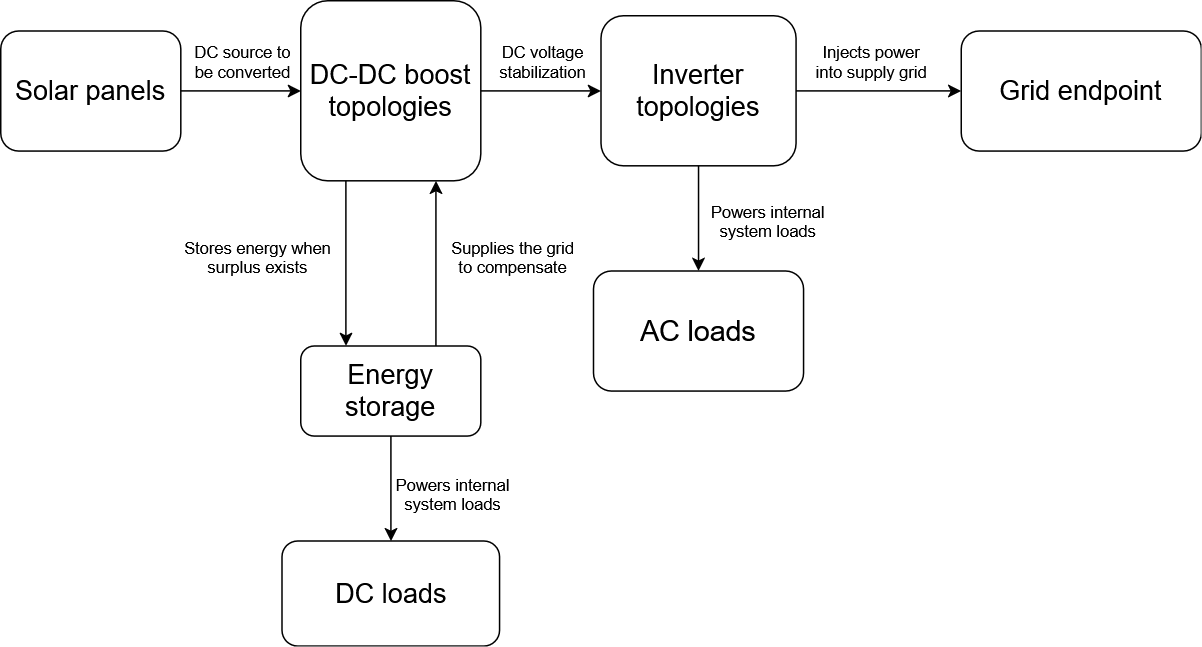
\includegraphics[width=\singlelongfigure]{\pics/models/pvsystem}\end{center}
    \caption{A typical configuration of a PV plant connected to a microgrid}
    \label{fig:pvsystem}
\end{figure}

As the paper focuses on inverter topologies, we assume the other system components behave within normal parameters and are not affected by significant defects.
The following sections will contain details about the chosen strategies for \gls{dc}-\gls{ac} conversion, topology used to implement this and the mathematical model of the circuit.

\section{The Anatomy of the Inverter System}
\label{sec:invsys}

\begin{figure}[!ht]
    \begin{center}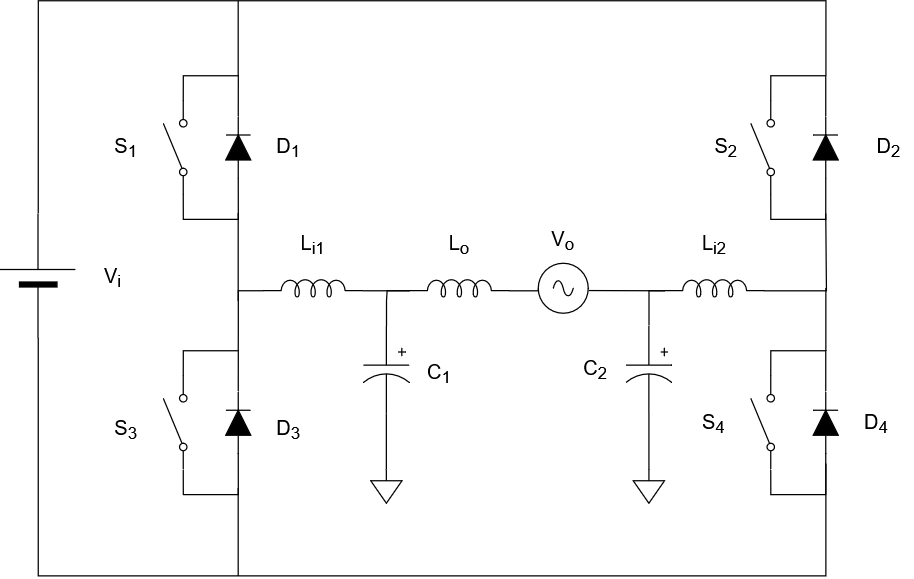
\includegraphics[width=\singlelongfigure]{\pics/models/hbridge}\end{center}
    \caption{The typical H-bridge structure with an LCL filter added at output}
    \label{fig:hbridge}
\end{figure}

Converting \gls{ac} current to \gls{dc} usually involves a simple diode rectifier, which is a passive circuit containing 4 diodes, meaning there isn't much to optimize in terms of electronic control besides physical construction.
However, the effort to do the opposite is considerably greater due to the fact that there is no circuit using only passive components that can modulate the voltage into a controlled sine wave.

\begin{table}[ht!]
\begin{tabular}{cccc}
\hline
State number & State description & Output voltage & Conducting components\\ 
 & & & for $i_o > 0$ \& $i_o < 0$ \\
\hline
1 & $S_1$ and $S_3$ open, $S_2$ and $S_4$ closed & $\frac{v_o}{2}$ & $S_1, S_3$ ; $D_1, D_3$\\
2 & $S_2$ and $S_4$ open, $S_1$ and $S_3$ closed & $-\frac{v_o}{2}$ & $S_2, S_4$ ; $D_2, D_4$\\
3 & $S_1$ and $S_2$ open, $S_3$ and $S_4$ closed & $0$ (short-circuit) & (not valid)\\
4 & $S_1$ and $S_2$ closed, $S_3$ and $S_4$ open & $0$ (short-circuit) & (not valid)\\
5 & $S_1$, $S_2$, $S_3$ and $S_4$ closed & $0$ (undefined) & $0$\\
\hline
\end{tabular}
\centering
\caption{All H-bridge states, with power outputs defined}
\label{tab:switchfunc}
\end{table}

The classic topology used for \gls{ac} power conversion is created using 4 switches in a formation known as a \gls{H-bridge} (example showcased in \figref{fig:hbridge}), with each half connected to one end of the load through a filter. \cite{rashid2013power}
Ideally, these switches are electrically controlled and don't possess any innate energy losses, however there are no such devices available with these characteristics.
The filter connected to each half bridge are designed to have 2 functions: they are energy storage devices that are used to create the sine wave injected into the grid, and they also reject high frequencies that are resulted from the residual energy consumption of the transistors' switching.
The principle behind converting the \gls{dc} current to \gls{ac} is by modulating the source voltage to match a carrier signal (in this case the load voltage) using a variable duty cycle \gls{pwm} signal that opens the transistors' gates.
These are switched alternatively to create both positive and negative voltages required for \gls{ac} forms, as shown in \tabref{tab:switchfunc}.

\section{Conduction Modes and Mathematical Model}
\label{sec:condmodes}

In any conversion switching circuit, there are two modes of conducting current through the filter inductors present in the topology, namely \gls{ccm} and \gls{dcm}.
These are related to how the current flowing through the circuit is stored into the inductor during any one switching cycle.
\gls{ccm} states that the current $i_{lx}$ should never drop to $0$ at any point in a cycle, whereas \gls{dcm} discharges the inductor completely until the time period elapses.
This comes with different advantages and disadvantages, such as requirements for inductor and capacitor sizes, presence of non-linear behaviour, conversion efficiency and maximum RMS current.
In the following subsections, there will be justifications provided for the usage of \gls{dcm} in the designed system.

\subsection{Justification for DCM Usage}
\label{subsec:justdcm}

Standard \gls{dc}-\gls{dc} and \gls{dc}-\gls{ac} conversion systems operate in \gls{ccm} due to its simplicity of writing a control algorithm for it as its behaviour is linear.
A simplified model of the system is presented in \figref{fig:ccmmodel}.

\begin{figure}[!ht]
    \begin{center}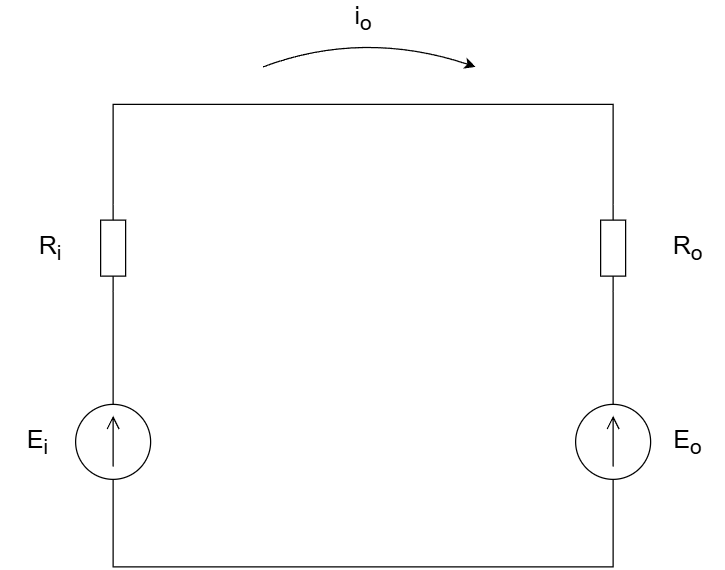
\includegraphics[width=\singlefigure]{\pics/models/ccmmodel}\end{center}
    \caption{Simplified model used for showcasing CCM}
    \label{fig:ccmmodel}
\end{figure}

The output voltage of the converter ($E_i$) depends on the duty cycle of the \gls{pwm} that drives the transistors as follows:
\begin{equation}
E_i = V_S \cdot q
\end{equation}
where $q$ is the duty cycle $[0, 1]$ of the \gls{pwm} signal and $V_S$ is the input source voltage that the system converts.
The output current $i_o$ would have the following form:
\begin{equation}
i_o = \frac{E_i - E_o}{R_i + R_o} = \frac{q \cdot V_S - E_o}{R_i + R_o}  
\end{equation}
Since the circuit is composed of 2 voltage sources placed in parallel and the internal resistances are ideally low in order to minimize energy losses, the output current is very sensitive to changes in the \gls{pwm} duty cycles.
As an example case, if we are to give values to each variable ($R_i = R_o = 1m\Omega, V_S = 12V, E_o = 3.6V$), $q$ would affect the output current as presented in \tabref{tab:ccmcur}.

\begin{table}[ht!]
\begin{center}
\begin{tabular}{|c|c|c|c|}
\hline
$i_o$ [A]&$E_i$ [V]&$q$ [\%]&PWM pulse length [ns]\\ \hline
0&3.600&30.000&120.000\\ \hline
50&3.700&30.833&123.333\\ \hline
-50&3.500&29.166&116.666\\ \hline
1&3.602&30.016&120.067\\ \hline
-1&3.598&29.983&119.933\\ \hline
0.1&3.6002&30.0016&120.0067\\ \hline
-0.1&3.5998&29.9983&119.9933\\ \hline
\end{tabular}
\end{center}
\caption{Experimental values provided using CCM control for the example system}
\label{tab:ccmcur}
\end{table}

It can be observed that the output current varies drastically even with small changes in the \gls{pwm} ratio, meaning that circuit control in this instance is a challenging task to achieve.
This would mean that many of the classic control methods used are inadequate unless the \gls{pwm} modulator can work with high resolutions.
Even if that is possible, as shown in \tabref{tab:ccmcur}, a small current change of $\pm 0.1A$ would require a change of $6.7ps$ in the \gls{pwm} pulse length, which is hard to achieve unless expensive hardware is utilized.
These kinds of frequencies cannot be achieved on microcontrollers, hardly on FPGAs, and are difficult to manage in circuit due to how susceptible to \gls{emi} the control signal is.

As mentioned previously at the beginning of \secref{sec:condmodes}, \gls{dcm} assumes that the energy stored in the filter inductor is fully discharged to the load at the end of each switching cycle.
This means that the system acts as a constant power source rather than a constant voltage source, which would mitigate the effects described previously.

\subsection{Explaining Converter Operation Under CCM vs DCM}
\label{subsec:ccmvsdcm}

\begin{figure}[!ht]
    \begin{center}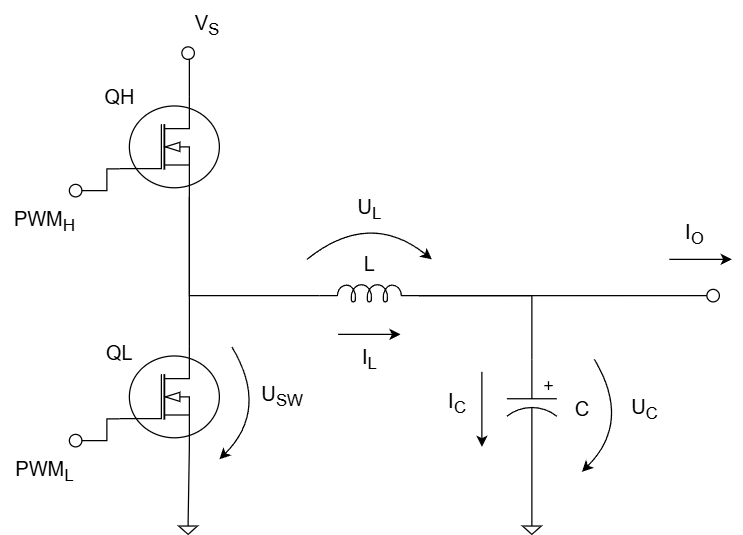
\includegraphics[width=\doublefigure]{\pics/models/bridgelc}\end{center}
    \caption{Simplified model of a half-bridge converter}
    \label{fig:bridgelc}
\end{figure}

\gls{H-bridge} topologies used in current conversions can be split up into two symmetrical half-bridge circuits as the control inputs are mirrored.
This part focuses on how each branch stores the converted input current ($I_o$) using the filter inductor on an LC filter.
A simplified version of such structure is presented in \figref{fig:bridgelc}.

In most cases where \gls{ccm} is used, the command signals $PWM_L$ and $PWM_H$ are generated similar to \figref{fig:pwmccm}, where $T_o$ is the constant period of the \gls{pwm} signal and $T_h$ is the pulse duration that controls the converter operation.
\begin{figure}[!ht]
    \begin{center}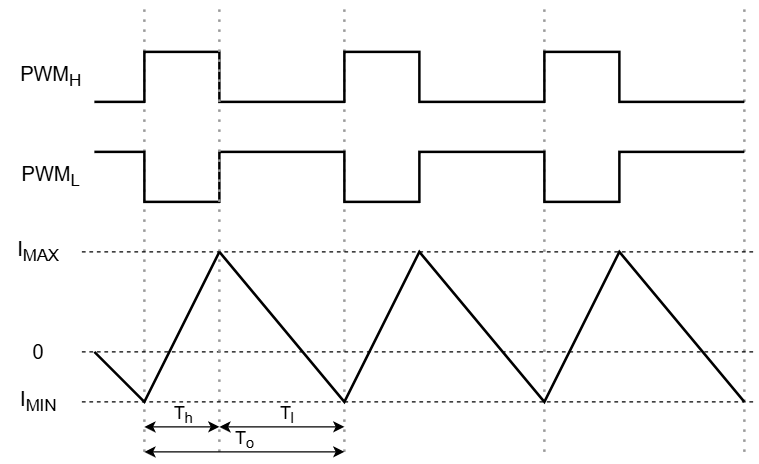
\includegraphics[width=\singlefigure]{\pics/models/pwmccm}\end{center}
    \caption{Current stored in the filter inductor under CCM}
    \label{fig:pwmccm}
\end{figure}

It can be observed that MOSFETs $QL$ and $QH$ (which is the most popular choice for small to medium voltage applications), are switched complementary.
Since MOSFETs allow current to pass in both directions when the conduction state is active, there are no restrictions  on the polarity of the current that passes through the inductor during switching period $T_o$.
Depending on the command signals $PWM_H$ and $PWM_L$, the converter can be found in one of these two states:
\begin{itemize}
    \item $PWM_H = 1$ and $PWM_L = 0$
    During this state, the switch node voltage $U_{SW} = V_S$ and the inductor changes according to:
    \begin{equation}
        \frac{dI_L}{dt} = \frac{U_L}{L} = \frac{U_{SW} - U_C}{L} = \frac{V_S - U_C}{L}
    \end{equation}
    The capacitor value is chosen large enough to assure a very small variation of its voltage during a switching period.
    As a result, the derivate of the inductor current is constant and has a positive value because $V_S > U_C$.
    This statement allows to approximate the inductor current as:
    \begin{equation}
        I_l(t) = I_{MIN} + \frac{dI_L}{dt} \cdot t = I_{MIN} + \frac{V_S - U_C}{L} \cdot t
    \end{equation}
    At the end of the $T_h$ time period where the converter transitions to the next state, the inductor current value will be as follows:
    \begin{equation}
        I_L(T_h) = I_{MIN} + \frac{V_S - U_C}{L} \cdot T_h = I_{MAX}
    \end{equation}
    
    \item $PWM_H = 0$ and $PWM_L = 1$
    During this stare, the switch node voltage $U_{SW} = 0$ and the inductor current changes according to:
    \begin{equation}
        \frac{dI_L}{dt} = \frac{U_L}{L} = \frac{U_{SW} - U_C}{L} = -\frac{U_C}{L}
    \end{equation}
    Assuming constant voltage across the capacitor, inductor current value can be approximated as:
    \begin{equation}
        I_L(t) = I_{MAX} + \frac{dI_L}{dt} \cdot (t - T_h) = I_{MAX} - \frac{U_C}{L} \cdot (t - T_h)
    \end{equation}
    At the end of the remaining time period $T_l$ where the next switching event will happen, the inductor current value will be:
    \begin{equation}
        I_L(T_h + T_l) = I_{MAX} - \frac{U_C}{L} \cdot T_l
    \end{equation}
\end{itemize}

In the steady state, $I_L(T_h + T_l) = I_{MIN}$ leads to:
\begin{equation}
    I_{MAX} - \frac{U_C}{L} \cdot T_l = I_{MIN}
\end{equation}
Replacing $I_{MAX}$ we obtain:
\begin{equation}
    I_{MIN} + \frac{V_S - U_C}{L} \cdot T_h - \frac{U_C}{L} \cdot T_l = I_{MIN}
\end{equation}
that gives the relation between voltages and switching time periods:
\begin{equation}
    \label{eq:ccmv2t}
    (V_S - U_C) \cdot T_h = U_C \cdot T_l
\end{equation}
If we consider that $T_l = T_o - T_h$, equation \eqref{eq:ccmv2t} becomes:
\begin{equation}
    (V_S - U_C) \cdot T_h = U_C \cdot (T_o - T_h)
\end{equation}
which in turn can be written as:
\begin{equation}
    \label{eq:finalccm}
    U_C = V_S \cdot \frac{T_h}{T_o} = q \cdot V_S
\end{equation}
Equation \eqref{eq:finalccm} shows that the half-bridge converter behaves as a controlled voltage source, and as presented in \subsecref{subsec:justdcm}, it makes current control substantially difficult.

To operate the converter in \gls{dcm} it is necessary to modify the gate control signals applied to the MOSFETs as follows:
\begin{itemize}
    \item if $I_o > 0$, the \gls{pwm} signal is applied only on the high-side transistor (QH)
    \item if $I_o < 0$, the \gls{pwm} signal is applied only on the low-side transistor (QL)
\end{itemize}
In \gls{dcm}, the inductor current is 0 at the beginning of each switching period and reaches the value of 0 before the end of switching period $T_o$.
If the \gls{pwm} signal is applied to the high-side transistor, the inductor current will have the evolution shown in \figref{fig:pwmdcm1}.

\begin{figure}[!ht]
    \begin{center}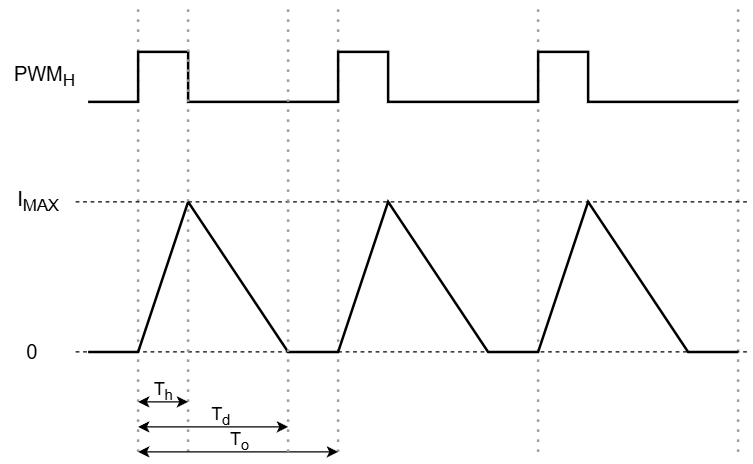
\includegraphics[width=\singlefigure]{\pics/models/pwmdcm1}\end{center}
    \caption{Current stored in the filter inductor under DCM using the high-side transistor}
    \label{fig:pwmdcm1}
\end{figure}

During the $T_h$ period, the switch node voltage $U_{SW} = V_S$ and the inductor current changes according to:
\begin{equation}
    I_L(t) = \frac{dI_L}{dt} \cdot t = \frac{V_S - U_C}{L} \cdot t
\end{equation}
At the end of the $T_h$ interval, the inductor current value will be:
\begin{equation}
    I_L(T_h) = \frac{V_S - U_C}{L} \cdot T_h = I_{MAX}
\end{equation}
After the MOSFET is turned off, the inductor current will flow through the internal body of the low-side transistor and the switch node voltage $U_{SW} = 0$ (assuming an ideal diode).
As a result, the inductor current will change according to:
\begin{equation}
    \begin{split}
        I_L(t) &= I_{MAX} + \frac{dI_L}{dt} \cdot(t - T_h)  \\
        &= I_{MAX} - \frac{U_C}{L} \cdot (t - T_h) \\
        &= \frac{V_S - U_C}{L} \cdot T_h - \frac{U_C}{L} \cdot (t - T_h)
    \end{split}
\end{equation}
When both time periods $T_h$ and $T_d$ ($t = T_h + T_d$) have elapsed, the inductor current becomes 0, which in turn would mean:
\begin{equation}
    \label{eq:lcurt}
    I_L(T_h + T_d) = \frac{V_S - U_C}{L} \cdot T_h - \frac{U_C}{L} \cdot [(T_h + T_d) - T_h] = 0
\end{equation}
From equation \eqref{eq:lcurt}, inductor discharge time $T_d$ can be written as:
\begin{equation}
    T_d = T_h \cdot \frac{V_S - U_C}{U_C}
\end{equation}
After this moment, the internal body diode will prevent the current through the inductor to drop at a negative value, therefore remaining at 0.

In the steady state, the output current $I_o$ is equal to the average value of the inductor current which is:
\begin{equation}
    \begin{split}
        I_o = (I_L)_{med} &= \frac{I_{MAX}}{2} \cdot \frac{T_h + T_d}{T_o} \\
        &= \left(\frac{V_S - U_C}{2 \cdot L} \cdot T_h\right) \cdot \frac{T_h}{T_o} \cdot \left(1 + \frac{V_S - U_C}{U_C}\right) \\
        &= \frac{V_S}{2 \cdot L \cdot T_o} \cdot \frac{V_S - U_C}{U_C} \cdot T_h^2
    \end{split}
\end{equation}

The condition for operating in \gls{dcm} is that $T_h + T_d < T_o$ that leads to:
\begin{equation}
    T_h + T_h \frac{V_S - U_C}{U_C} < T_o
\end{equation}
that imposes a maximum value for the transistor conduction period $T_h$:
\begin{equation}
    T_h < T_o \frac{U_C}{V_S}
\end{equation}
This condition limits the value of the output current to keep the converter to operate in \gls{dcm}:
\begin{equation}
    I_o < \frac{(V_S - U_C) \cdot U_C \cdot T_o}{2 \cdot L \cdot V_S} = \frac{V_S \cdot T_o}{2 \cdot L} \cdot \frac{U_C}{V_S} \cdot \left(1 - \frac{U_C}{V_S}\right)
\end{equation}
To ensure that the converter remains in \gls{dcm} regardless of the voltage across the capacitor, inductor value must be chosen as:
\begin{equation}
    L < L_{max} = \frac{V_S \cdot T_o}{2 \cdot I_o^{max}} \cdot min\left\{\frac{U_C^{min}}{V_S} \cdot \left(1 - \frac{U_C^{min}}{V_S}\right), \frac{U_C^{max}}{V_S} \cdot \left(1 - \frac{U_C^{max}}{V_S}\right)\right\}
\end{equation}

If the \gls{pwm} signal is applied to the low-side transistor, the inductor current will have the evolution described in \figref{fig:pwmdcm2}.

\begin{figure}[!ht]
    \begin{center}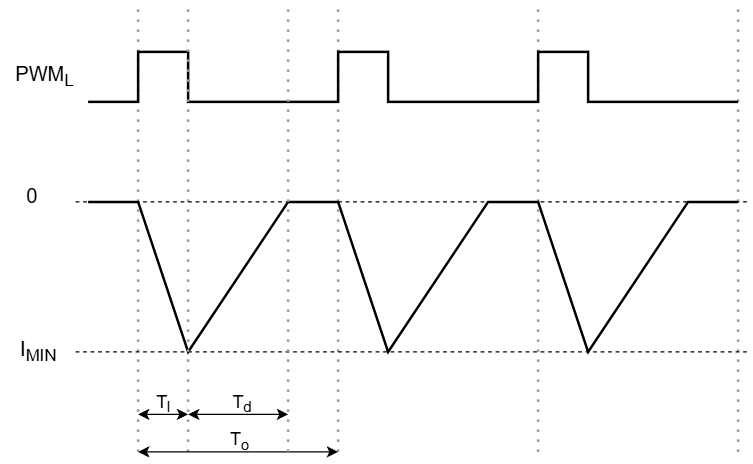
\includegraphics[width=\singlefigure]{\pics/models/pwmdcm2}\end{center}
    \caption{Current consumed by the filter inductor under DCM using the low-side transistor}
    \label{fig:pwmdcm2}
\end{figure}

During the $T_l$ period, the switch node voltage $U_{SW} = 0$ and the inductor current changes according to:
\begin{equation}
    I_L(t) = \frac{dI_L}{dt} \cdot t = -\frac{U_C}{L} \cdot
\end{equation}
At the end of the $T_l$ interval, the inductor current value will be:
\begin{equation}
I_L(T_l) = -\frac{U_C}{L} \cdot T_l = I_{MIN}
\end{equation}
After the MOSFET transistor is turned off, the inductor current will flow through the internal body diode of the high-side transistor and the switch node voltage $U_{SW}$ will become $V_S$ (assuming it is an ideal diode).
As a result, the inductor current will change according to:
\begin{equation}
    \begin{split}
        I_L(t) &= I_{MIN} + \frac{dI_L}{dt} \cdot (t - T_l) \\
        &= I_{MIN} + \frac{V_S - U_C}{L} \cdot (t - T_L) \\
        &= -\frac{U_C}{L} \cdot T_l + \frac{V_S - U_C}{L} \cdot (t - T_l)
    \end{split}
\end{equation}
When both time periods $T_h$ and $T_d$ ($t = T_h + T_d$) have elapsed, the inductor current becomes 0, which in turn would mean:
\begin{equation}
    I_L(T_l + T_d) = -\frac{U_C}{L} \cdot T_l + \frac{V_S - U_C}{L} \cdot [(T_l + T_d) - T_l] = 0
\end{equation}
From this equation, inductor discharge time $T_d$ can be obtained as:
\begin{equation}
    T_d = T_l \frac{U_C}{V_S - U_C}
\end{equation}
After $T_d$ elapses, the internal body diode will prevent the current through the inductor to raise beyond 0, therefore its value will remain zero.

In the steady state, the output current $I_o$ is equal to the average value of the inductor current which can be written as:
\begin{equation}
    \begin{split}
        I_o = (I_L)_{med} &= \frac{I_{MAX}}{2} \cdot \frac{T_l + T_d}{T_o} \\
        &= \left(-\frac{U_C}{2 \cdot L} \cdot T_l\right) \cdot \frac{T_l}{T_o} \cdot \left(1 + \frac{U_C}{V_S - U_C}\right) \\
        &= \frac{V_S}{2 \cdot L \cdot T_o} \cdot \frac{U_C}{V_S - U_C} \cdot T_l^2
    \end{split}
\end{equation}
In this case, the condition for operating in \gls{dcm} is $T_l + T_d < T_o$, which leads to:
\begin{equation}
    T_l + T_l \frac{U_C}{V_S - U_C} < T_O
\end{equation}
that imposes a maximum value for transistor conduction time period $T_l$:
\begin{equation}
    T_l < T_o \frac{V_S - U_C}{V_S}
\end{equation}
This condition leads to a maximum value for the negative output current to keep the converter operating in \gls{dcm}:
\begin{equation}
    I_o > -\frac{(V_S - U_C) \cdot U_C \cdot T_o}{2 \cdot L \cdot V_S} = -\frac{V_S \cdot T_o}{2 \cdot L} \cdot \frac{U_C}{V_S} \cdot \left(1 - \frac{U_C}{V_S}\right) 
\end{equation}
which has the same absolute value as the maximum current output when conducting the high-side transistor.
If the output current must be in the range of $[-I_o^{max}, +I_o^{max}]$, the condition that assures the operation in \gls{dcm} is:
\begin{equation}
    L < L_{max} = \frac{V_S \cdot T_o}{2 \cdot I_o^{max}} \cdot min\left\{\frac{U_C^{min}}{V_S} \cdot \left(1 - \frac{U_C^{min}}{V_S}\right), \frac{U_C^{max}}{V_S} \cdot \left(1 - \frac{U_C^{max}}{V_S}\right)\right\}
\end{equation}